\documentclass[11pt]{article}
\usepackage[margin=1in]{geometry}
\usepackage{mathpazo}
\usepackage{amsmath,amssymb}
\usepackage{microtype}
\usepackage{booktabs}
\usepackage{graphicx}
\usepackage[dvipsnames]{xcolor}
\usepackage{tikz}
\usetikzlibrary{positioning,arrows.meta,calc,fit,backgrounds,shapes.geometric}
\usepackage[compat=1.1.0]{tikz-feynman}
\usepackage[most]{tcolorbox}
\usepackage[font=small,labelfont=bf]{caption}
\usepackage{hyperref}
\hypersetup{colorlinks=true,linkcolor=MidnightBlue,citecolor=MidnightBlue,urlcolor=MidnightBlue}
\usepackage{cleveref}
\urlstyle{tt}
\def\UrlBreaks{\do\_\do/\do.}
\newcommand{\file}[1]{\nolinkurl{#1}}

% ---------------------------------------------------------------------------
\newcommand{\mhh}{m_{hh}}
\newcommand{\kl}{\kappa_\lambda}
\newcommand{\ct}{c_t}
\newcommand{\ctt}{c_{tt}}
\newcommand{\cggh}{c_{ggh}}
\newcommand{\cgghh}{c_{gghh}}
\newcommand{\bc}{\boldsymbol{c}}
\newcommand{\ba}{\boldsymbol{a}}
\newcommand{\bv}{\boldsymbol{v}}
\newcommand{\code}[1]{\texttt{#1}}

\definecolor{trainable}{HTML}{1B6CA8}
\definecolor{physics}{HTML}{2E933C}
\definecolor{datac}{HTML}{7B4EA3}

\newtcolorbox{keyidea}[1][]{enhanced,breakable,colback=physics!6,colframe=physics!70!black,
  fonttitle=\bfseries,title=#1,boxrule=0.6pt,arc=2pt,left=6pt,right=6pt}
\newtcolorbox{aside}[1][]{enhanced,breakable,colback=trainable!5,colframe=trainable!70!black,
  fonttitle=\bfseries,title=#1,boxrule=0.6pt,arc=2pt,left=6pt,right=6pt}

\title{\textbf{The \texttt{dihiggs} model}\\[4pt]
\large A physics-structured neural network for the HEFT di-Higgs mass spectrum}
\date{October 2026}

\begin{document}
\maketitle

\begin{abstract}
\noindent
This note explains, step by step, the model implemented in
\code{dihiggs/heftnet.py}. The goal is to predict the gluon-fusion di-Higgs
cross section in each bin of the di-Higgs invariant mass $\mhh$ as a function of
$\mhh$ and of five Wilson coefficients of the Higgs effective field theory (HEFT).
The central idea is to \emph{not} ask the neural network to learn what physics
already tells us: the dependence on the Wilson coefficients is a known polynomial
with 23 terms. The network learns only the 23 unknown functions of $\mhh$ that
multiply those terms. We first derive the polynomial, then describe the network,
the data, the training, and the testing, and end with some points worth noticing.
\end{abstract}

\tableofcontents

% ===========================================================================
\section{What we want to model, and why}
\label{sec:goal}

In gluon fusion, $gg \to hh$, new physics described by HEFT changes both the
size and the shape of the di-Higgs invariant-mass spectrum. The relevant part of
the HEFT Lagrangian is~\cite{alasfar}
\begin{equation}
  \mathcal{L}_{\text{HEFT}} \supset
  -m_t\Big(\ct\,\frac{h}{v} + \ctt\,\frac{h^2}{v^2}\Big)\bar t t
  - \kl\,\frac{m_h^2}{2v}\,h^3
  + \frac{\alpha_s}{8\pi}\Big(\cggh\,\frac{h}{v} + \cgghh\,\frac{h^2}{v^2}\Big)
    G^a_{\mu\nu}G^{a,\mu\nu},
  \label{eq:lagrangian}
\end{equation}
where $v \approx 246$~GeV. Each coefficient has a simple meaning:
\begin{center}
\begin{tabular}{lll}
\toprule
coefficient & interaction it controls & SM value\\
\midrule
$\kl \equiv c_{hhh}$ & Higgs self-coupling $hhh$ & 1\\
$\ct$   & top Yukawa coupling $t\bar t h$ & 1\\
$\ctt$  & contact coupling $t\bar t hh$ & 0\\
$\cggh$ & effective (point-like) coupling $ggh$ & 0\\
$\cgghh$& effective (point-like) coupling $gghh$ & 0\\
\bottomrule
\end{tabular}
\end{center}
We collect them into $\theta = (\kl, \ct, \ctt, \cggh, \cgghh)$.

We want a function
\begin{equation}
  \sigma(\mhh, \theta) = \text{cross section in a 15~GeV bin centred at } \mhh,
\end{equation}
valid everywhere in a broad region of the 5-dimensional $\theta$ space.
Such a function lets us \emph{reweight} existing simulated events to any other
$\theta$, instead of running a new simulation for every point, and it is an
ingredient of the simulation-based construction of confidence sets in $\theta$
that motivates this project~\cite{lee,alkadhim}.

\Cref{fig:spectra} shows four of the simulated spectra. Notice how different they
are: their sizes span three orders of magnitude, some fall steeply from threshold,
one peaks near 700~GeV, and spectrum~(b) has a sharp dip near 330~GeV, a sign of
destructive interference between different contributions to the amplitude.
The model has to describe all of these with one set of parameters.

\begin{figure}[t]
  \centering
  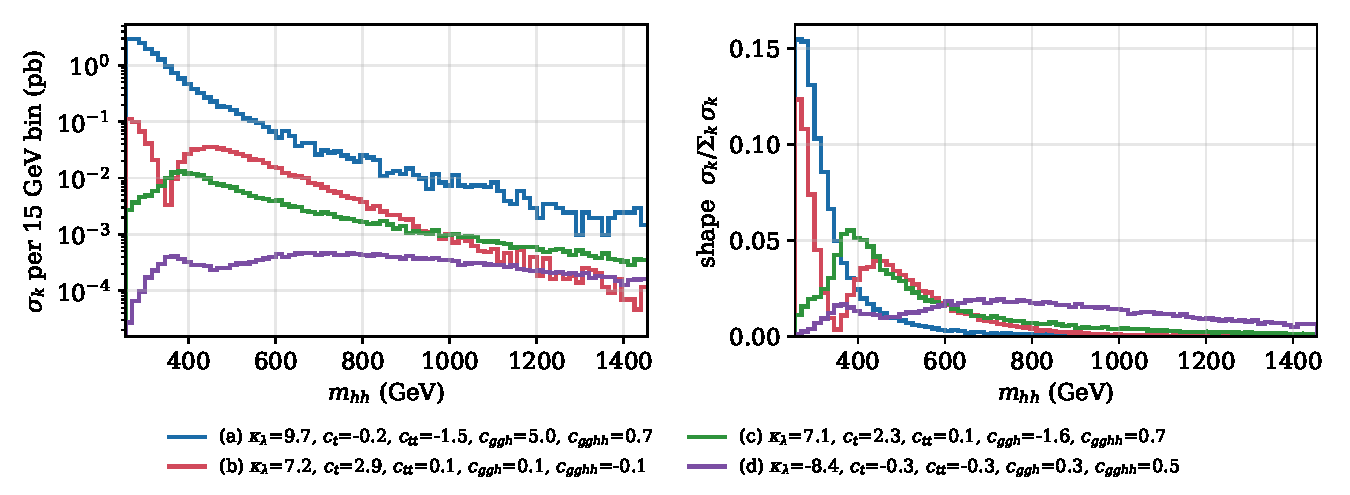
\includegraphics[width=\textwidth]{spectra.pdf}
  \caption{Four POWHEG spectra from the held-out test set, chosen to show the
  range of shapes. Left: cross section per 15~GeV bin (log scale). Right: the same
  spectra divided by their totals, so that only the shapes are compared.}
  \label{fig:spectra}
\end{figure}

% ===========================================================================
\section{The physics: why $\sigma$ is a polynomial in $\theta$}
\label{sec:physics}

\subsection{The amplitude is linear in the couplings}

At leading order (LO) there are five classes of Feynman diagrams for
$gg\to hh$ in HEFT (\cref{fig:feynman}). Each class contains exactly one
combination of couplings: two top Yukawa vertices in the box, a Yukawa vertex
and the self-coupling in the top-loop triangle, and so on. Therefore the full
amplitude is a \emph{linear} combination of five fixed sub-amplitudes,
\begin{equation}
  \mathcal{M} = \ct^2\,\mathcal{M}_1 + \ct\kl\,\mathcal{M}_2 + \ctt\,\mathcal{M}_3
  + \cggh\kl\,\mathcal{M}_4 + \cgghh\,\mathcal{M}_5
  \;\equiv\; \sum_{i=1}^{5} v_i(\theta)\,\mathcal{M}_i ,
  \label{eq:amp}
\end{equation}
with
\begin{equation}
  \bv(\theta) = \big(\ct^2,\; \ct\kl,\; \ctt,\; \cggh\kl,\; \cgghh\big).
  \label{eq:v}
\end{equation}
The sub-amplitudes $\mathcal{M}_i$ depend on the kinematics (on $\mhh$ and the
scattering angle) but \emph{not} on $\theta$. All of the $\theta$ dependence is in the
five numbers $v_i$.

\begin{figure}[t]
\centering
\tikzfeynmanset{every vertex={/tikz/inner sep=0pt}}
\newcommand{\diaglabel}[2]{\node[below=2pt, align=center, font=\small] at (#1) {#2};}
% (1) box
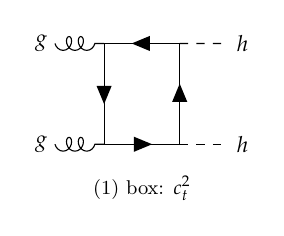
\begin{tikzpicture}[scale=0.8, transform shape]
  \begin{feynman}
    \vertex (g1) at (0,1.6) {$g$};
    \vertex (g2) at (0,0) {$g$};
    \vertex (a) at (1.0,1.6);
    \vertex (b) at (1.0,0);
    \vertex (c) at (2.2,0);
    \vertex (d) at (2.2,1.6);
    \vertex (h1) at (3.2,1.6) {$h$};
    \vertex (h2) at (3.2,0) {$h$};
    \diagram* {
      (g1) -- [gluon] (a), (g2) -- [gluon] (b),
      (a) -- [fermion] (b) -- [fermion] (c) -- [fermion] (d) -- [fermion] (a),
      (d) -- [scalar] (h1), (c) -- [scalar] (h2),
    };
  \end{feynman}
  \node[font=\small] at (1.6,-0.7) {(1) box: $\ct^2$};
\end{tikzpicture}\hfill
% (2) triangle with self-coupling
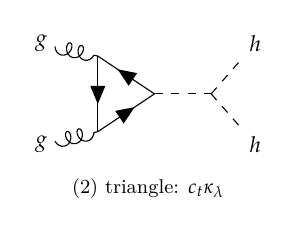
\begin{tikzpicture}[scale=0.8, transform shape]
  \begin{feynman}
    \vertex (g1) at (0,1.6) {$g$};
    \vertex (g2) at (0,0) {$g$};
    \vertex (a) at (0.9,1.4);
    \vertex (b) at (0.9,0.2);
    \vertex (c) at (1.8,0.8);
    \vertex (v) at (2.7,0.8);
    \vertex (h1) at (3.4,1.6) {$h$};
    \vertex (h2) at (3.4,0) {$h$};
    \diagram* {
      (g1) -- [gluon] (a), (g2) -- [gluon] (b),
      (a) -- [fermion] (b) -- [fermion] (c) -- [fermion] (a),
      (c) -- [scalar] (v),
      (v) -- [scalar] (h1), (v) -- [scalar] (h2),
    };
  \end{feynman}
  \node[font=\small] at (1.7,-0.7) {(2) triangle: $\ct\kl$};
\end{tikzpicture}\hfill
% (3) triangle with tthh
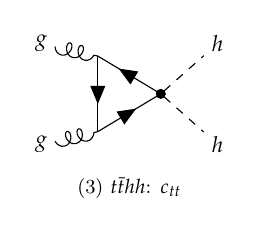
\begin{tikzpicture}[scale=0.8, transform shape]
  \begin{feynman}
    \vertex (g1) at (0,1.6) {$g$};
    \vertex (g2) at (0,0) {$g$};
    \vertex (a) at (0.9,1.4);
    \vertex (b) at (0.9,0.2);
    \vertex[dot, minimum size=4pt] (c) at (1.9,0.8) {};
    \vertex (h1) at (2.8,1.6) {$h$};
    \vertex (h2) at (2.8,0) {$h$};
    \diagram* {
      (g1) -- [gluon] (a), (g2) -- [gluon] (b),
      (a) -- [fermion] (b) -- [fermion] (c) -- [fermion] (a),
      (c) -- [scalar] (h1), (c) -- [scalar] (h2),
    };
  \end{feynman}
  \node[font=\small] at (1.4,-0.7) {(3) $t\bar thh$: $\ctt$};
\end{tikzpicture}\hfill
% (4) ggh contact + self coupling
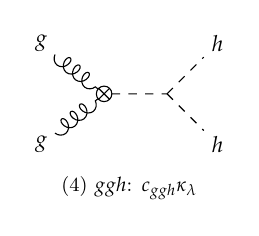
\begin{tikzpicture}[scale=0.8, transform shape]
  \begin{feynman}
    \vertex (g1) at (0,1.6) {$g$};
    \vertex (g2) at (0,0) {$g$};
    \vertex[crossed dot, minimum size=7pt] (c) at (1.0,0.8) {};
    \vertex (v) at (2.0,0.8);
    \vertex (h1) at (2.8,1.6) {$h$};
    \vertex (h2) at (2.8,0) {$h$};
    \diagram* {
      (g1) -- [gluon] (c), (g2) -- [gluon] (c),
      (c) -- [scalar] (v),
      (v) -- [scalar] (h1), (v) -- [scalar] (h2),
    };
  \end{feynman}
  \node[font=\small] at (1.4,-0.7) {(4) $ggh$: $\cggh\kl$};
\end{tikzpicture}\hfill
% (5) gghh contact
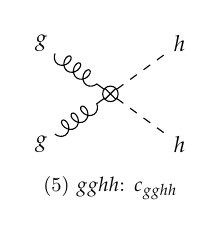
\begin{tikzpicture}[scale=0.8, transform shape]
  \begin{feynman}
    \vertex (g1) at (0,1.6) {$g$};
    \vertex (g2) at (0,0) {$g$};
    \vertex[crossed dot, minimum size=7pt] (c) at (1.1,0.8) {};
    \vertex (h1) at (2.2,1.6) {$h$};
    \vertex (h2) at (2.2,0) {$h$};
    \diagram* {
      (g1) -- [gluon] (c), (g2) -- [gluon] (c),
      (c) -- [scalar] (h1), (c) -- [scalar] (h2),
    };
  \end{feynman}
  \node[font=\small] at (1.1,-0.7) {(5) $gghh$: $\cgghh$};
\end{tikzpicture}
\caption{The five classes of LO diagrams for $gg\to hh$ in HEFT and the
coupling combination each one carries. Solid lines are top quarks, dashed lines
Higgs bosons; the dot is the $t\bar thh$ contact vertex and the crossed dots are
the point-like gluon--Higgs vertices of \cref{eq:lagrangian}.}
\label{fig:feynman}
\end{figure}

\subsection{Squaring the amplitude gives 15 terms}

A cross section is proportional to $|\mathcal{M}|^2$. Squaring
\cref{eq:amp} gives
\begin{equation}
  |\mathcal{M}|^2 = \sum_{i=1}^{5}\sum_{j=1}^{5} v_i\, v_j\,
  \mathrm{Re}\big(\mathcal{M}_i\mathcal{M}_j^*\big).
\end{equation}
Now integrate over everything except $\mhh$ (the scattering angle, and the
parton distributions), and over one 15~GeV bin. Because the $v_i$ do not depend on
the kinematics, they come out of the integral:
\begin{equation}
  \sigma(\mhh,\theta) = \sum_{i\le j} v_i(\theta)\,v_j(\theta)\, K_{ij}(\mhh),
  \qquad
  K_{ij}(\mhh) \propto \int \mathrm{Re}\big(\mathcal{M}_i\mathcal{M}_j^*\big)\,
  d(\text{everything but } \mhh).
  \label{eq:quadratic}
\end{equation}
$K$ is a symmetric $5\times 5$ matrix of functions of $\mhh$, so it has
$5\cdot 6/2 = 15$ independent entries. The 15 products $v_iv_j$, written out in the
couplings, are the first 15 monomials in \cref{tab:monomials}. The diagonal
entries $K_{ii}$ are squared magnitudes and so are non-negative; the off-diagonal
entries are \emph{interference} terms and can have either sign. Negative
interference is what produces dips such as the one in spectrum~(b) of
\cref{fig:spectra}.

\subsection{Next-to-leading order adds 8 more terms}

The training data were generated with POWHEG at next-to-leading order (NLO) in
QCD. At NLO new diagram classes appear, and the polynomial grows from 15 to 23
terms~\cite{alasfar}. One way to see where the 8 extra terms come from is to
consider the NLO diagrams in which each Higgs boson attaches to the gluons through
its own single-Higgs vertex, either a top loop ($\propto\ct$) or the point-like
$ggh$ vertex ($\propto\cggh$). Their coupling factors are
$\boldsymbol{w} = (\ct^2,\;\ct\cggh,\;\cggh^2)$. Interfering these with the LO
amplitude gives products $w_a v_i$. The products with $w_1=\ct^2$ reproduce LO
monomials, but those with $\ct\cggh$ and $\cggh^2$ give exactly the 8 new monomials
16--23 of \cref{tab:monomials}.

\begin{keyidea}[Key idea]
For \emph{every} $\mhh$ the cross section is a fixed polynomial in $\theta$:
\begin{equation}
  \boxed{\;\sigma(\mhh,\theta) = \sum_{i=1}^{23} c_i(\theta)\, a_i(\mhh)
  = \bc(\theta)\cdot\ba(\mhh)\;}
  \label{eq:factorised}
\end{equation}
The 23 monomials $c_i(\theta)$ are \emph{known exactly} (\cref{tab:monomials}).
Only the 23 functions $a_i(\mhh)$ are unknown. They are the integrated (and
NLO-corrected) interference kernels $K_{ij}$. The coupling dependence and the
kinematic dependence \emph{factorise}.
\end{keyidea}

The LHC Higgs Working Group determines the $a_i$ (called $dA_i$ there) one bin at a
time with a least-squares fit~\cite{alasfar}. The \code{dihiggs} model instead
represents them as smooth functions of $\mhh$ given by a neural network.

% ===========================================================================
\section{The model}
\label{sec:model}

\subsection{Architecture}

\Cref{fig:architecture} shows the whole model. It has two branches that meet
in a dot product.

\begin{figure}[t]
\centering
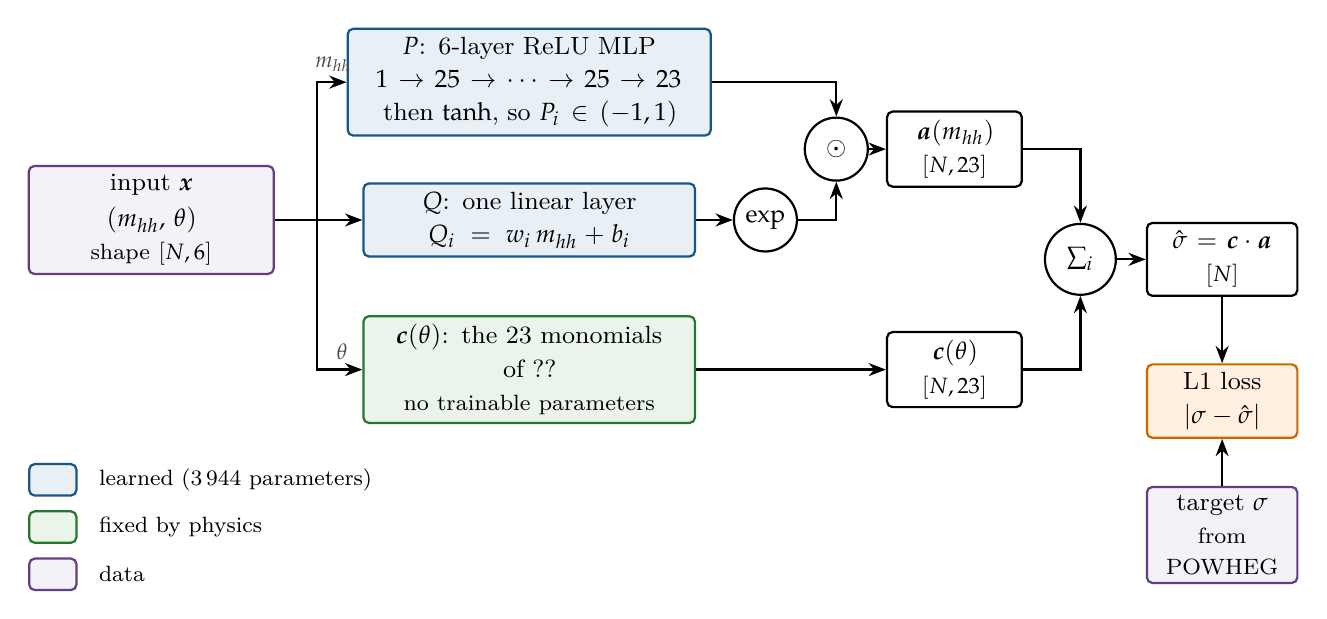
\begin{tikzpicture}[
  font=\small,
  >={Stealth[length=2.2mm]},
  box/.style={draw, rounded corners=2pt, thick, align=center, minimum height=9mm,
              inner sep=3pt},
  train/.style={box, fill=trainable!10, draw=trainable!80!black},
  phys/.style={box, fill=physics!10, draw=physics!80!black},
  dat/.style={box, fill=datac!8, draw=datac!80!black},
  op/.style={circle, draw, thick, minimum size=8mm, inner sep=0pt, fill=white},
  lab/.style={font=\footnotesize, text=black!70},
]
% ---- nodes (explicit coordinates, in cm) ----
\node[dat, text width=29mm] (x) at (1.55,0)
  {input $\boldsymbol{x}$\\[2pt] $(\mhh,\,\theta)$\\[1pt]\footnotesize shape $[N,6]$};
\coordinate (s) at (3.65,0);
\node[train, text width=44mm] (P) at (6.35,1.75)
  {$P$: 6-layer ReLU MLP\\[1pt]
   $1\to25\to\cdots\to25\to23$\\[1pt]
   then $\tanh$, so $P_i\in(-1,1)$};
\node[train, text width=40mm] (Q) at (6.35,0.0)
  {$Q$: one linear layer\\[1pt] $Q_i = w_i\,\mhh + b_i$};
\node[op] (exp) at (9.35,0.0) {$\exp$};
\node[op] (mul) at (10.25,0.9) {$\odot$};
\node[box, text width=15mm, fill=white] (a) at (11.75,0.9)
  {$\ba(\mhh)$\\[1pt]\footnotesize $[N,23]$};
\node[phys, text width=40mm] (c) at (6.35,-1.9)
  {$\bc(\theta)$: the 23 monomials\\[1pt] of \cref{tab:monomials}\\[1pt]
   \footnotesize no trainable parameters};
\node[box, text width=15mm, fill=white] (cv) at (11.75,-1.9)
  {$\bc(\theta)$\\[1pt]\footnotesize $[N,23]$};
\node[op, minimum size=9mm] (dot) at (13.35,-0.5) {$\sum_i$};
\node[box, text width=17mm, fill=white] (sig) at (15.15,-0.5)
  {$\hat\sigma=\bc\cdot\ba$\\[1pt]\footnotesize $[N]$};
\node[box, text width=17mm, fill=orange!12, draw=orange!80!black] (loss) at (15.15,-2.3)
  {L1 loss\\[1pt] $|\sigma-\hat\sigma|$};
\node[dat, text width=17mm] (t) at (15.15,-4.0)
  {target $\sigma$\\[1pt]\footnotesize from POWHEG};

% ---- arrows ----
\draw[thick] (x.east) -- (s);
\draw[->, thick] (s) |- node[lab, pos=0.78, above]{$\mhh$} (P.west);
\draw[->, thick] (s) -- (Q.west);
\draw[->, thick] (s) |- node[lab, pos=0.78, above]{$\theta$} (c.west);
\draw[->, thick] (Q) -- (exp);
\draw[->, thick] (P.east) -| (mul.north);
\draw[->, thick] (exp.east) -| (mul.south);
\draw[->, thick] (mul) -- (a);
\draw[->, thick] (c) -- (cv);
\draw[->, thick] (a.east) -| (dot.north);
\draw[->, thick] (cv.east) -| (dot.south);
\draw[->, thick] (dot) -- (sig);
\draw[->, thick] (sig) -- (loss);
\draw[->, thick] (t) -- (loss);

% ---- legend ----
\node[train, minimum height=4mm, minimum width=6mm, inner sep=0pt] (l1) at (0.3,-3.3) {};
\node[right=1.5mm of l1, font=\footnotesize, anchor=west] {learned (3\,944 parameters)};
\node[phys, minimum height=4mm, minimum width=6mm, inner sep=0pt] (l2) at (0.3,-3.9) {};
\node[right=1.5mm of l2, font=\footnotesize, anchor=west] {fixed by physics};
\node[dat, minimum height=4mm, minimum width=6mm, inner sep=0pt] (l3) at (0.3,-4.5) {};
\node[right=1.5mm of l3, font=\footnotesize, anchor=west] {data};
\end{tikzpicture}
\caption{The \code{HEFTNet} model. Each input row, $\boldsymbol{x}=(\mhh,\theta)$ with
$\theta=(\kl,\ct,\ctt,\cggh,\cgghh)$, is split. The mass $\mhh$ feeds
two small networks, $P$ and $Q$, which give the 23 functions
$a_i(\mhh)=P_i(\mhh)\,e^{Q_i(\mhh)}$. The Wilson coefficients $\theta$ feed the
23 known monomials $c_i(\theta)$. The prediction is the dot product $\bc\cdot\ba$,
which is compared with the POWHEG cross section using the absolute (L1) loss.
Blue boxes are learned; the green box is fixed by physics.}
\label{fig:architecture}
\end{figure}

\paragraph{The physics branch, $\bc(\theta)$.} The five Wilson coefficients are
turned into the 23-component vector of monomials in \cref{tab:monomials}. This
branch has no trainable parameters; it is simply \cref{eq:quadratic} and its NLO
extension written as code (\code{torch.column\_stack} in \code{HEFTNet.forward}).

\paragraph{The learned branch, $\ba(\mhh)$.} The mass alone determines the 23
functions, through
\begin{equation}
  a_i(\mhh) = P_i(\mhh)\; e^{\,Q_i(\mhh)}, \qquad i = 1,\dots,23,
  \label{eq:PQ}
\end{equation}
where
\begin{itemize}
  \item $P$ is a fully connected network with one input and 23 outputs:
  a $1\to25$ layer, five $25\to25$ layers, each followed by a ReLU, and a final
  $25\to23$ layer followed by $\tanh$. This is 3\,898 parameters.
  \item $Q$ is a single linear layer with one input and 23 outputs,
  $Q_i(\mhh) = w_i\,\mhh + b_i$, which is 46 parameters.
\end{itemize}

\begin{aside}[Why the product $P\,e^{Q}$?]
Because $Q_i$ is linear, $e^{Q_i(\mhh)} = e^{b_i}\,e^{w_i\mhh}$. The two factors
have separate jobs, and $P_i$ has a third:
\begin{itemize}
  \item $e^{b_i}$ sets the \emph{overall size} of $a_i$. The 23 functions can
  differ in magnitude by orders of magnitude. Learning $b_i$, a logarithm of the
  size, is far easier for gradient descent than learning a tiny or huge number
  directly.
  \item $e^{w_i\mhh}$ supplies an \emph{exponential fall-off} with $\mhh$, which
  is the gross behaviour of the spectra in \cref{fig:spectra}.
  \item $P_i\in(-1,1)$ supplies the \emph{shape and the sign}. A sign is needed
  because the interference functions can be negative. The $\tanh$ keeps $P_i$
  bounded, so the magnitude is always controlled by $e^{Q_i}$.
\end{itemize}
In short, $e^{Q}$ is a simple learned envelope and $P$ is a learned, bounded
correction to it.
\end{aside}

\paragraph{The prediction.} For an input row
$\boldsymbol{x}=(\mhh,\kl,\ct,\ctt,\cggh,\cgghh)$ the output is
\begin{equation}
  \hat\sigma(\boldsymbol{x}) = \sum_{i=1}^{23} c_i(\theta)\,P_i(\mhh)\,e^{Q_i(\mhh)} .
\end{equation}
\Cref{tab:shapes} follows the tensors through \code{HEFTNet.forward} for a
batch of $N$ rows.

\begin{table}[h]
\centering
\begin{tabular}{lll}
\toprule
step in \code{forward} & tensor & shape\\
\midrule
input batch & $\boldsymbol{x}$ & $[N,6]$\\
split columns & $\mhh,\kl,\ct,\ctt,\cggh,\cgghh$ & six of $[N]$\\
monomials (\code{column\_stack}) & $\bc(\theta)$ & $[N,23]$\\
reshape mass & $\mhh$ & $[N,1]$\\
networks & $P(\mhh)$, $Q(\mhh)$ & $[N,23]$ each\\
coefficients (\code{coeffs}) & $\ba = P\odot e^{Q}$ & $[N,23]$\\
row-wise dot product & $\hat\sigma = \sum_i c_i a_i$ & $[N]$\\
\bottomrule
\end{tabular}
\caption{Tensor shapes in \code{HEFTNet.forward}.}
\label{tab:shapes}
\end{table}

\subsection{What the structure buys us}

\begin{enumerate}
  \item \textbf{Exact dependence on the couplings.} For any $\theta$, including
  values outside the training region, the prediction has exactly the right
  polynomial form. Only the $a_i$ are approximated. A generic network with all six
  inputs would have to discover this polynomial from data and could not
  extrapolate it.
  \item \textbf{A one-dimensional learning problem.} The network sees only
  $\mhh$. Learning 23 smooth functions of one variable is much easier than
  learning one function of six variables.
  \item \textbf{Interpretable outputs.} The $a_i(\mhh)$ are physical quantities,
  namely the interference kernels, and can be plotted and compared with the
  binned $dA_i$ of Ref.~\cite{alasfar}. \code{heft\_test.ipynb} plots them.
  \item \textbf{A continuous function of $\mhh$.} The model can be evaluated at
  any $\mhh$, not just at bin centres.
\end{enumerate}

% ===========================================================================
\section{The data}
\label{sec:data}

\paragraph{Spectra.} The file \file{data/powheg_total_gauss_params_13TeV.csv.gz}
contains 4\,999 POWHEG NLO spectra at $\sqrt{s}=13$~TeV. Each row holds one
parameter point $\theta$ and the cross section in pb in 100 bins of 15~GeV. The
parameter points are scattered roughly as Gaussians centred on the SM point, with
standard deviations of about 5 for $\kl$ and about 2 for the other four
coefficients. Hence the name ``wide Gauss''.

\paragraph{Bins and the mass variable.} Bins 0--15 are empty, and bin 16
straddles the threshold $\mhh = 2m_h = 250$~GeV: the POWHEG histograms start at
0~GeV with 15~GeV bins, so bin $k$ covers $[15k,\,15(k+1))$~GeV. \code{heft\_prepare\_data.ipynb} keeps bins
17--96, that is $255 \le \mhh < 1455$~GeV, and maps them to a dimensionless
variable on the unit interval with bins of width $0.01$:
\begin{equation}
  x = \frac{\mhh - 255~\text{GeV}}{1500~\text{GeV}}, \qquad
  x_k = \frac{k - 17 + \tfrac12}{100}, \quad k = 17,\dots,96 .
\end{equation}
In the code, the column called \code{mhh} holds this $x$, which runs from $0.005$
to $0.795$. Keeping the network input of order one is good practice.

\paragraph{From spectra to training rows.} After shuffling the spectra:
\begin{itemize}
  \item the first 500 are set aside, untouched, as the test set
  (\file{heft_wide_gauss_testdata_13TeV.csv});
  \item each of the remaining 4\,499 spectra is ``diced'' into 80 rows
  $(\theta, x_k, \sigma_k)$, one per bin. Rows with $\sigma_k=0$ are dropped and
  the rows are shuffled, leaving 357\,958 rows
  (\file{heft_wide_gauss_traindata_13TeV.csv.gz}).
\end{itemize}
Dicing is what makes the problem a standard regression: every row is one
example, input $\boldsymbol{x}=(x_k,\theta)$ and target $\sigma_k$.

% ===========================================================================
\section{Training}
\label{sec:training}

\paragraph{Splits.} \code{heft\_train.ipynb} splits the 357\,958 rows into
301\,056 for training ($=147$ batches of 2\,048), 6\,902 for validation, and 50\,000
for a quick test. A random subset of the training rows, of the same size as the
validation set, is used to compare training and validation losses, which is a
check for overfitting.

\paragraph{Loss.} The parameters $\omega$ of $P$ and $Q$ are found by minimising
the empirical risk with the absolute (L1) loss,
\begin{equation}
  R(\omega) = \frac{1}{M}\sum_{m=1}^{M}
  \big|\,\sigma_m - \bc(\theta_m)\cdot\ba(x_m;\omega)\,\big| .
\end{equation}
The minimiser of the expected absolute loss is the conditional
\emph{median} of the target given the input. With the squared loss it would be the
conditional mean. For simulated spectra the target is a deterministic function
of the input up to Monte Carlo noise, so both would give essentially the same
function. The L1 loss is less sensitive to occasional large fluctuations.

\paragraph{Optimisation.} Adam with mini-batches of 2\,048 rows for 200\,000
iterations, about 1\,360 passes through the training set. The learning rate starts
at $2\times10^{-3}$ and is halved every 50\,000 iterations, giving four steps:
$2\times10^{-3}$, $10^{-3}$, $5\times10^{-4}$, $2.5\times10^{-4}$.
Every 100 iterations the average losses on the training subset and the validation
set are recorded. The parameters are saved whenever the validation loss drops by
more than 1.5\% below its best value so far.

% ===========================================================================
\section{Testing}
\label{sec:testing}

\code{heft\_test.ipynb} reloads the saved parameters and does two things.
\begin{enumerate}
  \item It plots the 23 learned functions $a_i(\mhh)$, the quantities the network
  was built to find.
  \item For each of the 500 held-out spectra it evaluates $\hat\sigma$ at the 80
  bin centres and overlays the result on the POWHEG histogram. None of these
  parameter points was used in training. The test is therefore a direct check of
  how well the model \emph{interpolates in $\theta$}, which is the property needed
  for reweighting.
\end{enumerate}

% ===========================================================================
\section{Points worth noticing}
\label{sec:notes}

\begin{itemize}
  \item \textbf{Positivity is not enforced.} Nothing forces $\hat\sigma\ge0$, nor
  the diagonal kernels to be non-negative. A well-trained model should be very
  close to non-negative where there are data, but it is worth checking near the
  dips.
  \item \textbf{The absolute loss weights rows by their size.} The targets span
  roughly $10^{-6}$ to $30$~pb per bin. An absolute error of $10^{-4}$~pb is
  negligible for a large spectrum but a large \emph{relative} error for a small
  one. Training is therefore dominated by the larger cross sections. A relative or
  logarithmic loss would weight the spectra more evenly, at the price of different
  statistical properties.
  \item \textbf{Identifiability.} At a fixed $\mhh$, $\sigma$ is linear in the 23
  unknowns $a_i$. They are determined uniquely only if the 23 monomials evaluated
  at the training points are linearly independent. With thousands of
  random $\theta$ points spread widely, as here, they are. With a few points close
  to the SM, they would not be.
\end{itemize}

% ===========================================================================
\appendix
\section{The 23 monomials}
\label{app:monomials}

\begin{table}[h]
\centering
\small
\renewcommand{\arraystretch}{1.3}
\begin{tabular}{rll@{\hspace{2.5em}}rll}
\toprule
$i$ & $c_i(\theta)$ & origin & $i$ & $c_i(\theta)$ & origin\\
\midrule
1  & $\ct^4$            & $v_1v_1$ & 13 & $\kl^2\cggh\ct$      & $v_2v_4$\\
2  & $\ctt^2$           & $v_3v_3$ & 14 & $\cgghh\ct\kl$       & $v_2v_5$\\
3  & $\ct^2\kl^2$       & $v_2v_2$ & 15 & $\cggh\cgghh\kl$     & $v_4v_5$\\
4  & $\cggh^2\kl^2$     & $v_4v_4$ & 16 & $\ct^3\cggh$         & $(\ct\cggh)\,v_1$\\
5  & $\cgghh^2$         & $v_5v_5$ & 17 & $\ct\ctt\cggh$       & $(\ct\cggh)\,v_3$\\
6  & $\ctt\ct^2$        & $v_1v_3$ & 18 & $\ct\cggh^2\kl$      & $(\ct\cggh)\,v_4$\\
7  & $\kl\ct^3$         & $v_1v_2$ & 19 & $\ct\cggh\cgghh$     & $(\ct\cggh)\,v_5$\\
8  & $\ct\kl\ctt$       & $v_2v_3$ & 20 & $\ct^2\cggh^2$       & $\cggh^2\,v_1$\\
9  & $\cggh\kl\ctt$     & $v_3v_4$ & 21 & $\ctt\cggh^2$        & $\cggh^2\,v_3$\\
10 & $\ctt\cgghh$       & $v_3v_5$ & 22 & $\cggh^3\kl$         & $\cggh^2\,v_4$\\
11 & $\cggh\kl\ct^2$    & $v_1v_4$ & 23 & $\cggh^2\cgghh$      & $\cggh^2\,v_5$\\
12 & $\cgghh\ct^2$      & $v_1v_5$ &    &                      & \\
\bottomrule
\end{tabular}
\caption{The monomials in the order used in \code{heftnet.py}, which is also the
order of Eq.~(4.1) of Ref.~\cite{alasfar}. Terms 1--15 are the products $v_iv_j$
of the LO coupling factors in \cref{eq:v} and suffice at LO. Terms 16--23 appear
at NLO. Their ``origin'' column shows them as an NLO coupling factor
($\ct\cggh$ or $\cggh^2$) times an LO factor $v_i$, as described in
\cref{sec:physics}. In the code, \code{klambda} $=\kl$, \code{CT} $=\ct$,
\code{CTT} $=\ctt$, \code{CGGH} $=\cggh$, \code{CGGHH} $=\cgghh$.}
\label{tab:monomials}
\end{table}

% ===========================================================================
\begin{thebibliography}{9}
\bibitem{alasfar} L.~Alasfar \emph{et al.}, \emph{Effective Field Theory
  descriptions of Higgs boson pair production}, LHC Higgs Working Group public
  note, \href{https://arxiv.org/abs/2304.01968}{arXiv:2304.01968}
  (included in this repository as \code{docs/theory.pdf}).
\bibitem{lee} N.~Dalmasso, L.~Masserano, D.~Zhao, R.~Izbicki and A.~B.~Lee,
  \emph{Likelihood-free frequentist inference: bridging classical statistics
  and machine learning for reliable simulator-based inference},
  \href{https://arxiv.org/abs/2107.03920}{arXiv:2107.03920}.
\bibitem{alkadhim} A.~Al~Kadhim \emph{et al.}, \emph{Amortized simulation-based
  frequentist inference for tractable and intractable likelihoods},
  Mach.\ Learn.: Sci.\ Technol.\ (2024),
  \href{https://iopscience.iop.org/article/10.1088/2632-2153/ad218e}{doi:10.1088/2632-2153/ad218e}.
\end{thebibliography}

\end{document}
